
%% bare_conf.tex
%% V1.3
%% 2007/01/11
%% by Michael Shell
%% See:
%% http://www.michaelshell.org/
%% for current contact information.
%%
%% This is a skeleton file demonstrating the use of IEEEtran.cls
%% (requires IEEEtran.cls version 1.7 or later) with an IEEE conference paper.
%%
%% Support sites:
%% http://www.michaelshell.org/tex/ieeetran/
%% http://www.ctan.org/tex-archive/macros/latex/contrib/IEEEtran/
%% and
%% http://www.ieee.org/

%%*************************************************************************
%% Legal Notice:
%% This code is offered as-is without any warranty either expressed or
%% implied; without even the implied warranty of MERCHANTABILITY or
%% FITNESS FOR A PARTICULAR PURPOSE! 
%% User assumes all risk.
%% In no event shall IEEE or any contributor to this code be liable for
%% any damages or losses, including, but not limited to, incidental,
%% consequential, or any other damages, resulting from the use or misuse
%% of any information contained here.
%%
%% All comments are the opinions of their respective authors and are not
%% necessarily endorsed by the IEEE.
%%
%% This work is distributed under the LaTeX Project Public License (LPPL)
%% ( http://www.latex-project.org/ ) version 1.3, and may be freely used,
%% distributed and modified. A copy of the LPPL, version 1.3, is included
%% in the base LaTeX documentation of all distributions of LaTeX released
%% 2003/12/01 or later.
%% Retain all contribution notices and credits.
%% ** Modified files should be clearly indicated as such, including  **
%% ** renaming them and changing author support contact information. **
%%
%% File list of work: IEEEtran.cls, IEEEtran_HOWTO.pdf, bare_adv.tex,
%%                    bare_conf.tex, bare_jrnl.tex, bare_jrnl_compsoc.tex
%%*************************************************************************

% *** Authors should verify (and, if needed, correct) their LaTeX system  ***
% *** with the testflow diagnostic prior to trusting their LaTeX platform ***
% *** with production work. IEEE's font choices can trigger bugs that do  ***
% *** not appear when using other class files.                            ***
% The testflow support page is at:
% http://www.michaelshell.org/tex/testflow/



% Note that the a4paper option is mainly intended so that authors in
% countries using A4 can easily print to A4 and see how their papers will
% look in print - the typesetting of the document will not typically be
% affected with changes in paper size (but the bottom and side margins will).
% Use the testflow package mentioned above to verify correct handling of
% both paper sizes by the user's LaTeX system.
%
% Also note that the "draftcls" or "draftclsnofoot", not "draft", option
% should be used if it is desired that the figures are to be displayed in
% draft mode.
%
\documentclass[conference]{IEEEtran}
% Add the compsoc option for Computer Society conferences.
%
% If IEEEtran.cls has not been installed into the LaTeX system files,
% manually specify the path to it like:
% \documentclass[conference]{../sty/IEEEtran}





% Some very useful LaTeX packages include:
% (uncomment the ones you want to load)


% *** MISC UTILITY PACKAGES ***
%
%\usepackage{ifpdf}
% Heiko Oberdiek's ifpdf.sty is very useful if you need conditional
% compilation based on whether the output is pdf or dvi.
% usage:
% \ifpdf
%   % pdf code
% \else
%   % dvi code
% \fi
% The latest version of ifpdf.sty can be obtained from:
% http://www.ctan.org/tex-archive/macros/latex/contrib/oberdiek/
% Also, note that IEEEtran.cls V1.7 and later provides a builtin
% \ifCLASSINFOpdf conditional that works the same way.
% When switching from latex to pdflatex and vice-versa, the compiler may
% have to be run twice to clear warning/error messages.






% *** CITATION PACKAGES ***
%
%\usepackage{cite}
% cite.sty was written by Donald Arseneau
% V1.6 and later of IEEEtran pre-defines the format of the cite.sty package
% \cite{} output to follow that of IEEE. Loading the cite package will
% result in citation numbers being automatically sorted and properly
% "compressed/ranged". e.g., [1], [9], [2], [7], [5], [6] without using
% cite.sty will become [1], [2], [5]--[7], [9] using cite.sty. cite.sty's
% \cite will automatically add leading space, if needed. Use cite.sty's
% noadjust option (cite.sty V3.8 and later) if you want to turn this off.
% cite.sty is already installed on most LaTeX systems. Be sure and use
% version 4.0 (2003-05-27) and later if using hyperref.sty. cite.sty does
% not currently provide for hyperlinked citations.
% The latest version can be obtained at:
% http://www.ctan.org/tex-archive/macros/latex/contrib/cite/
% The documentation is contained in the cite.sty file itself.






% *** GRAPHICS RELATED PACKAGES ***
%
\ifCLASSINFOpdf
  \usepackage[pdftex]{graphicx}
  % declare the path(s) where your graphic files are
  \graphicspath{{../pdf/}{../jpeg/}}
  % and their extensions so you won't have to specify these with
  % every instance of \includegraphics
  \DeclareGraphicsExtensions{.pdf,.jpeg,.png}
\else
  % or other class option (dvipsone, dvipdf, if not using dvips). graphicx
  % will default to the driver specified in the system graphics.cfg if no
  % driver is specified.
  % \usepackage[dvips]{graphicx}
  % declare the path(s) where your graphic files are
  % \graphicspath{{../eps/}}
  % and their extensions so you won't have to specify these with
  % every instance of \includegraphics
  % \DeclareGraphicsExtensions{.eps}
\fi
% graphicx was written by David Carlisle and Sebastian Rahtz. It is
% required if you want graphics, photos, etc. graphicx.sty is already
% installed on most LaTeX systems. The latest version and documentation can
% be obtained at: 
% http://www.ctan.org/tex-archive/macros/latex/required/graphics/
% Another good source of documentation is "Using Imported Graphics in
% LaTeX2e" by Keith Reckdahl which can be found as epslatex.ps or
% epslatex.pdf at: http://www.ctan.org/tex-archive/info/
%
% latex, and pdflatex in dvi mode, support graphics in encapsulated
% postscript (.eps) format. pdflatex in pdf mode supports graphics
% in .pdf, .jpeg, .png and .mps (metapost) formats. Users should ensure
% that all non-photo figures use a vector format (.eps, .pdf, .mps) and
% not a bitmapped formats (.jpeg, .png). IEEE frowns on bitmapped formats
% which can result in "jaggedy"/blurry rendering of lines and letters as
% well as large increases in file sizes.
%
% You can find documentation about the pdfTeX application at:
% http://www.tug.org/applications/pdftex





% *** MATH PACKAGES ***
%
%\usepackage[cmex10]{amsmath}
% A popular package from the American Mathematical Society that provides
% many useful and powerful commands for dealing with mathematics. If using
% it, be sure to load this package with the cmex10 option to ensure that
% only type 1 fonts will utilized at all point sizes. Without this option,
% it is possible that some math symbols, particularly those within
% footnotes, will be rendered in bitmap form which will result in a
% document that can not be IEEE Xplore compliant!
%
% Also, note that the amsmath package sets \interdisplaylinepenalty to 10000
% thus preventing page breaks from occurring within multiline equations. Use:
%\interdisplaylinepenalty=2500
% after loading amsmath to restore such page breaks as IEEEtran.cls normally
% does. amsmath.sty is already installed on most LaTeX systems. The latest
% version and documentation can be obtained at:
% http://www.ctan.org/tex-archive/macros/latex/required/amslatex/math/





% *** SPECIALIZED LIST PACKAGES ***
%
%\usepackage{algorithmic}
% algorithmic.sty was written by Peter Williams and Rogerio Brito.
% This package provides an algorithmic environment fo describing algorithms.
% You can use the algorithmic environment in-text or within a figure
% environment to provide for a floating algorithm. Do NOT use the algorithm
% floating environment provided by algorithm.sty (by the same authors) or
% algorithm2e.sty (by Christophe Fiorio) as IEEE does not use dedicated
% algorithm float types and packages that provide these will not provide
% correct IEEE style captions. The latest version and documentation of
% algorithmic.sty can be obtained at:
% http://www.ctan.org/tex-archive/macros/latex/contrib/algorithms/
% There is also a support site at:
% http://algorithms.berlios.de/index.html
% Also of interest may be the (relatively newer and more customizable)
% algorithmicx.sty package by Szasz Janos:
% http://www.ctan.org/tex-archive/macros/latex/contrib/algorithmicx/




% *** ALIGNMENT PACKAGES ***
%
%\usepackage{array}
% Frank Mittelbach's and David Carlisle's array.sty patches and improves
% the standard LaTeX2e array and tabular environments to provide better
% appearance and additional user controls. As the default LaTeX2e table
% generation code is lacking to the point of almost being broken with
% respect to the quality of the end results, all users are strongly
% advised to use an enhanced (at the very least that provided by array.sty)
% set of table tools. array.sty is already installed on most systems. The
% latest version and documentation can be obtained at:
% http://www.ctan.org/tex-archive/macros/latex/required/tools/


%\usepackage{mdwmath}
%\usepackage{mdwtab}
% Also highly recommended is Mark Wooding's extremely powerful MDW tools,
% especially mdwmath.sty and mdwtab.sty which are used to format equations
% and tables, respectively. The MDWtools set is already installed on most
% LaTeX systems. The lastest version and documentation is available at:
% http://www.ctan.org/tex-archive/macros/latex/contrib/mdwtools/


% IEEEtran contains the IEEEeqnarray family of commands that can be used to
% generate multiline equations as well as matrices, tables, etc., of high
% quality.


%\usepackage{eqparbox}
% Also of notable interest is Scott Pakin's eqparbox package for creating
% (automatically sized) equal width boxes - aka "natural width parboxes".
% Available at:
% http://www.ctan.org/tex-archive/macros/latex/contrib/eqparbox/





% *** SUBFIGURE PACKAGES ***
%\usepackage[tight,footnotesize]{subfigure}
% subfigure.sty was written by Steven Douglas Cochran. This package makes it
% easy to put subfigures in your figures. e.g., "Figure 1a and 1b". For IEEE
% work, it is a good idea to load it with the tight package option to reduce
% the amount of white space around the subfigures. subfigure.sty is already
% installed on most LaTeX systems. The latest version and documentation can
% be obtained at:
% http://www.ctan.org/tex-archive/obsolete/macros/latex/contrib/subfigure/
% subfigure.sty has been superceeded by subfig.sty.



%\usepackage[caption=false]{caption}
%\usepackage[font=footnotesize]{subfig}
% subfig.sty, also written by Steven Douglas Cochran, is the modern
% replacement for subfigure.sty. However, subfig.sty requires and
% automatically loads Axel Sommerfeldt's caption.sty which will override
% IEEEtran.cls handling of captions and this will result in nonIEEE style
% figure/table captions. To prevent this problem, be sure and preload
% caption.sty with its "caption=false" package option. This is will preserve
% IEEEtran.cls handing of captions. Version 1.3 (2005/06/28) and later 
% (recommended due to many improvements over 1.2) of subfig.sty supports
% the caption=false option directly:
%\usepackage[caption=false,font=footnotesize]{subfig}
%
% The latest version and documentation can be obtained at:
% http://www.ctan.org/tex-archive/macros/latex/contrib/subfig/
% The latest version and documentation of caption.sty can be obtained at:
% http://www.ctan.org/tex-archive/macros/latex/contrib/caption/




% *** FLOAT PACKAGES ***
%
%\usepackage{fixltx2e}
% fixltx2e, the successor to the earlier fix2col.sty, was written by
% Frank Mittelbach and David Carlisle. This package corrects a few problems
% in the LaTeX2e kernel, the most notable of which is that in current
% LaTeX2e releases, the ordering of single and double column floats is not
% guaranteed to be preserved. Thus, an unpatched LaTeX2e can allow a
% single column figure to be placed prior to an earlier double column
% figure. The latest version and documentation can be found at:
% http://www.ctan.org/tex-archive/macros/latex/base/



%\usepackage{stfloats}
% stfloats.sty was written by Sigitas Tolusis. This package gives LaTeX2e
% the ability to do double column floats at the bottom of the page as well
% as the top. (e.g., "\begin{figure*}[!b]" is not normally possible in
% LaTeX2e). It also provides a command:
%\fnbelowfloat
% to enable the placement of footnotes below bottom floats (the standard
% LaTeX2e kernel puts them above bottom floats). This is an invasive package
% which rewrites many portions of the LaTeX2e float routines. It may not work
% with other packages that modify the LaTeX2e float routines. The latest
% version and documentation can be obtained at:
% http://www.ctan.org/tex-archive/macros/latex/contrib/sttools/
% Documentation is contained in the stfloats.sty comments as well as in the
% presfull.pdf file. Do not use the stfloats baselinefloat ability as IEEE
% does not allow \baselineskip to stretch. Authors submitting work to the
% IEEE should note that IEEE rarely uses double column equations and
% that authors should try to avoid such use. Do not be tempted to use the
% cuted.sty or midfloat.sty packages (also by Sigitas Tolusis) as IEEE does
% not format its papers in such ways.





% *** PDF, URL AND HYPERLINK PACKAGES ***
%
%\usepackage{url}
% url.sty was written by Donald Arseneau. It provides better support for
% handling and breaking URLs. url.sty is already installed on most LaTeX
% systems. The latest version can be obtained at:
% http://www.ctan.org/tex-archive/macros/latex/contrib/misc/
% Read the url.sty source comments for usage information. Basically,
% \url{my_url_here}.





% *** Do not adjust lengths that control margins, column widths, etc. ***
% *** Do not use packages that alter fonts (such as pslatex).         ***
% There should be no need to do such things with IEEEtran.cls V1.6 and later.
% (Unless specifically asked to do so by the journal or conference you plan
% to submit to, of course. )


% correct bad hyphenation here
\hyphenation{op-tical net-works semi-conduc-tor}


\begin{document}



%
% paper title
% can use linebreaks \\ within to get better formatting as desired
\title{Customer Community Identification from Community Detection Graph in E-Commerce}


% author names and affiliations
% use a multiple column layout for up to three different
% affiliations
\author{\IEEEauthorblockN{Ihsan Satriawan}
\IEEEauthorblockA{School of Electronic Engineering and Informatics\\
Institute of Technology Bandung\\
Bandung, Indonesia\\
ihsan.satriawan.20[at]gmail.com}
\and
\IEEEauthorblockN{G.A. Putri Saptawati}
\IEEEauthorblockA{School of Electronic Engineering and Informatics\\
Institute of Technology Bandung\\
Bandung, Indonesia\\
putri[at]informatika.org}}

% make the title area
\maketitle


\begin{abstract}
%\boldmath
In business today, it is very important to be able to identify customer behavior, and arrange strategy based that information. In this research, we propose graph modeling, customer community for e-commerce data, and use concept TF-IDF (Term Frequency-Inverse Document Frequency) in text mining domain to identify customer community. In this research, we associate term as product which is bought by customer and document as community or customer. With this approach, we can get information from customer community, where contains typical product from each community. This information can useful for arrange promotion product to customer community.
\end{abstract}
% IEEEtran.cls defaults to using nonbold math in the Abstract.
% This preserves the distinction between vectors and scalars. However,
% if the conference you are submitting to favors bold math in the abstract,
% then you can use LaTeX's standard command \boldmath at the very start
% of the abstract to achieve this. Many IEEE journals/conferences frown on
% math in the abstract anyway.

\begin{IEEEkeywords}
Community Detection, Graph, Community Identification, TF-IDF
\end{IEEEkeywords}




% For peer review papers, you can put extra information on the cover
% page as needed:
% \ifCLASSOPTIONpeerreview
% \begin{center} \bfseries EDICS Category: 3-BBND \end{center}
% \fi
%
% For peerreview papers, this IEEEtran command inserts a page break and
% creates the second title. It will be ignored for other modes.
\IEEEpeerreviewmaketitle



\section{Introduction}
E-commerce is one of the sectors in trading which is rapidly growing. Research by consulting firm A.T. Kearney in 2015, showed that Indonesia had potential in E-commerce between USD
25 - 30 billion.

\begin{figure}[h]
\centering
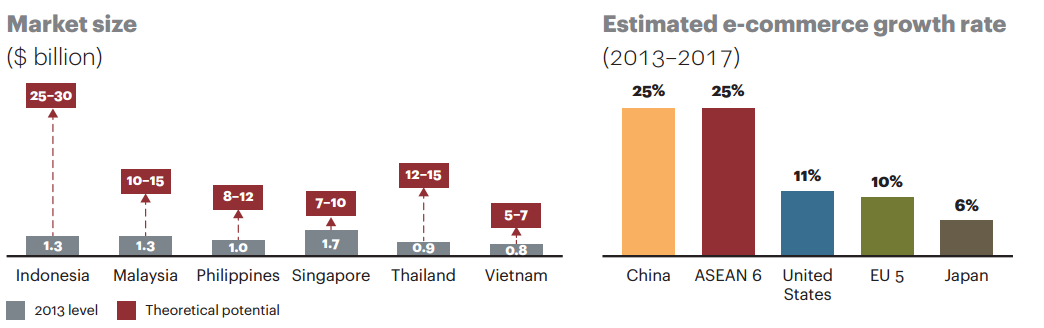
\includegraphics[width=\columnwidth]{figure/marketpotency}
\caption{ASEAN's Market Potency}
\label{market_potency}
\end{figure}

Based on those potential value, no wonder if Indonesia has many E-commerce companies like Tokopedia, Bukalapak, Hijup, MatahaMall, etc. This condition make every company must give better service than other and make their customer satisfied if want to survive. Company must be able to understand their customer behavior when bought product and arrange marketing strategy based on that information \cite{Tsiptsis}.

Data mining is crucial for extracting and identifying useful information from a large amount of data \cite{Ahmed}. E-Commerce company operate databases in a long way, such that all transactions are stored in chronological order. A record-of-transaction database typically contains the transaction date and the products bought in the course of a given transaction. Usually, each record also contains an customer ID, particularly when the purchase was made using a credit card \cite{Ahmed}.

Networks have become ubiquitous as data from many different disciplines can be naturally mapped to graph structures \cite{Malliaros}. An interesting feature that real networks present is the clustering or community structure property, under which the graph topology is organized into modules commonly called community detection. Informally, Community detection is to partition the set of network nodes into multiple groups such that the nodes within a group are connected densely, but connections between groups are sparse \cite{Malliaros}

In this research, we have use another approach to extract useful information from data e-commerce. We modelled data e-commerce as graph and apply community detection method to get customer community and extract useful information from community.



\section{Related Work}
There are some research about community detection. The Girvan-Newman (GN) algorithm proposed by Girvan and Newman \cite{Newman} exploits the concept of edge betweenness, which is a measure of the centrality and influence of an edge in a network. Community detection in weighted graph based on twitter data use GN algorithm by Mairisha \cite{Mairisha}. Based on the time complexity of some of the methods for large networks, a detection method with a small time complexity was required. The best method that was found was the detection method first proposed by Newman and Girvan \cite{Kameyama}

However, community in networks depends on what we define relation each node. We still need to identify each community. In order to perform this task, another procedure is required, a different property must be used to identify the communities. In many cases, a possible choice is to use the semantics of a community as a unique property. For example, with the TF-IDF technique apply by Uchida et al \cite{Uchida}, an attempt was made to characterize the communities detected in a blogosphere. Specific topics discussed in each community were found, and it was shown that the communities can be identified by such specific topics. Thus, it can be considered that semantics is a useful property for identifying a community

Research by Uchida et all, use TF-IDF to identify communities detected without apply feature reduction and term weighted. it's potential error in choose term to identify topic in entries/document \cite{Dai}. Feature reduction and term weighted is part of feature selection. Feature selection becomes very important, because it features the words chosen results reduction features and patterns formed determine the precision of word weighting results grouping news \cite{Dai,DaiX}


\section{Methodology}
In this research, we apply Term Frequency-Inverse Document Frequency (TF-IDF) and Term Contribution (TC) to identify customer community. The steps of the research process as shown in figure \ref{overall_methodology}

\begin{figure}[h]
\centering
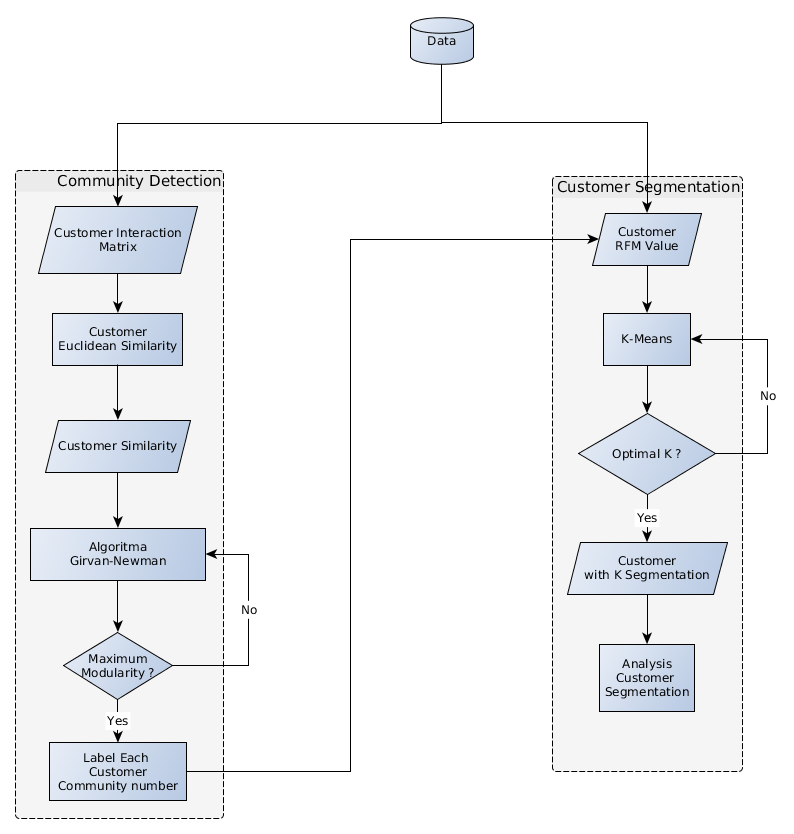
\includegraphics[width=\columnwidth]{figure/overall_methodology}
\caption{Overall methodology}
\label{overall_methodology}
\end{figure}

\subsection{Data Preprocessing}
This step is selects related data that we acquired from e-commerce to be used in case study of discovering customer community and then pre-processes data which is an important step. Data preprocessing eliminates irrelevant data by some methods such as data integration, data transformation, and data reduction. Prepared data is shown at Table \ref{tab:sample_data_preprocessing_result}

\begin{table}[h]
\renewcommand{\arraystretch}{1.3}
\caption{Sample Data Preprocessing Result}
\label{tab:sample_data_preprocessing_result}
\centering
\begin{tabular}{c|c|c}
    \hline
    ID-Sender  &  ID-Receiver & Total Frequency Interaction\\
    \hline
    79424 & 78112 & 2\\
    \hline
    64554 & 43874 & 2\\
    \hline
    48249 & 21061 & 18\\
    \hline
\end{tabular}
\end{table}

\subsection{Graph Modeling}
We construct a network regarding customers as nodes and interaction each customers (column "Total Frequency Interaction" in Table \ref{tab:sample_data_preprocessing_result}) as undirected edges ,although interaction is directed, we consider the network undirected, making each edge bidirectional. For make each edge bidirectional, we apply symmetrizing, equation \ref{eq:symmetrizing} show that formula \cite{Gopalakrishnan}

\begin{equation}
	\label{eq:symmetrizing}
	\bar{A} = (A + A^T)/2
\end{equation}

\begin{figure}[h]
\centering
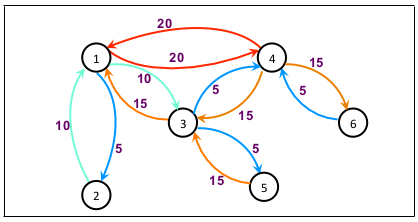
\includegraphics[width=\columnwidth, height=3cm,keepaspectratio]{figure/bidirectional_edge}
\caption{Example of a weighted directed network}
\label{bidirectional_edge}
\end{figure}

\begin{figure}[h]
\centering
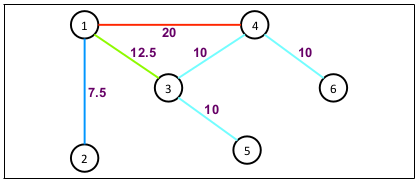
\includegraphics[width=\columnwidth, height=3cm,keepaspectratio]{figure/undirected_edge}
\caption{Symmetrized version of the weighted directed network shown in Fig \ref{bidirectional_edge}}
\label{undirected_edge}
\end{figure}

\subsection{Community Detection}
The GN algorithm is a divisive hierarchical clustering algorithm exploiting the concept of edge betweenness \cite{Newman}. Three methods were proposed for the calculation of edge betweenness. Among them, the shortest-path method typically shows the best results. The edge betweenness of an edge is informally the number of shortest paths between pairs of nodes that pass through it. Since communities are loosely connected by a few “intergroup” edges, all shortest paths between different communities must pass through one of these few edges. Then, those edges connecting communities will have high edge betweenness. Thus, the communities are detected by eliminating such edges repeatedly.

To decide how much community divide in networks, measure of quality of divide in networks, which  call the modularity. The modularity is, up to a multiplicative constant, the number of edges falling within groups minus the expected number in an equivalent network with edges placed at random, equation \ref{eq:modularity_GN} show formula from modularity GN \cite{Newman}

\begin{equation}
	\label{eq:modularity_GN}
    Q = \frac{1}{2m} \Sigma_{vw} [A_{vw} - \frac{(k_{v}k_{w})}{2m}] \sigma(c_{v}c_{w})
\end{equation}

Good community detection on graph have big modularity score, otherwise poor community detection have small modularity score. Modularity score calculate on every create new community. If formed x community, than there is x modularity score. The number of communities that have the highest modularity score indicates the formation of the community in accordance with the actual reality.
\subsection{Identify Community}
Inspired from use TF-IDF to summarization document and TC and Z-score as feature reduction in domain text mining \cite{Munggaran}, we apply this concept to identify customer community. In our case, we associate term as product which is bought by customer and document as community or customer.

\begin{figure}[h]
\centering

\includegraphics[width=\columnwidth, height=3cm,keepaspectratio]{figure/identify_community}
\caption{Flow Identify Community}
\label{bidirectional_edge}
\end{figure}

\subsubsection{Term Frequency-Inverse Document Frequency}
TF-IDF stands for "Term Frequency, Inverse Document Frequency". It is a way to score the importance of words (or "terms") in a document based on how frequently they appear across multiple documents \cite{Lan}. TF-IDF contain two value, term frequency \((tf)\) and inverse document frequency \((idf)\), where \(tf\) is number of occurence of term in document (in our case, number of occurance of product bought in community or customer) and \(idf\) is number of document containing term (in our case, number of community or customer bought product). Value of \(idf\) follow equation \ref{eq:idf} and equation \ref{eq:tf-idf} shown formula for calculate TF-IDF.

\begin{equation}
	\label{eq:idf}
    idf(t) = \log  \frac{D}{df(t)}
\end{equation}

\begin{equation}
	\label{eq:tf-idf}
    TFxIDF(t,d) = tf(t,d) idf(t,d)
\end{equation}



\subsubsection{Term Contribution}
TC influences the value of word frequency \((tf)\) as a component score. TC score calculate from term frequency (TF) and Inverse Document Frequency (IDF) \cite{Liu}

\begin{equation}
	\label{eq:TC_score}
    TC(t) = \Sigma_{i,j \cap i \neq j} f(t,d_{i}) X f(t,d_{j})
\end{equation}

where \(f(t,d)\) represents the \(tf*idf\) weight of term in document \(d\) whereas \(i\) and \(j\) are document \(i\) document \(j\) and \(i\) not equal \(j\). \(\Sigma f(t,d)\) is sum TF-IDF from term \(t\) in document \(d\)

\subsubsection{Z-score}
Assuming that the important words are selected based set of words that have a high score and dominant among other, it can be determined by the difference in distance between score. Z-score calculating a value of the average deviation and density of data \cite{Olga}. This can be made possible as a solution for the elimination or  word removal. This is more flexible and can be used for different datasets. The optimal parameters can be identified at a middle value (zero). Words that have a score greater than zero \((\geq 0)\) is an important word and relevant, otherwise,  the word is not an important word and irrelevant and will be removed.

\begin{equation}
	\label{eq:Z_score}
    Z = \frac{x - \bar{x}}{\sigma}
\end{equation}

\section{Experimental Result}
As described in the previous section, we will organize the experiment results follows with the step of methodology in the previous section.

\subsection{Data Preprocessing}
This research used database from one e-commerce mus-limah in Indonesia for last 1 years (2015-2016). After making a selection of data, the records which include missing values and inaccurate values are removed, and eliminated the redundant attributes. The dataset contains 88,103 records data interaction and 178,276 records data transaction. Data interaction is interaction customer to customer for transfer point reward.


\subsection{Graph Modeling}
We build graph object with node is set of customer and undirected edge is interaction each customer with mean frequency interaction between customer as the edge weight. Generated graph is visualize as show in Fig \ref{Graph_customer_interaction}

\begin{figure}[h]
\centering
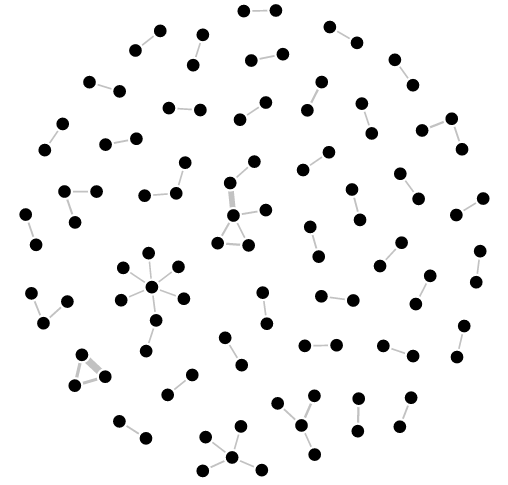
\includegraphics[width=\columnwidth, height=5cm,keepaspectratio]{figure/graph_awal}
\caption{Flow Identify Community}
\label{Graph_customer_interaction}
\end{figure}

\subsection{Community Detection}
For each community detection process iteration, modularity score become quality measure. Table \ref{tab:modularity_score} show modularity score for each number of community formed. Because 42 community have highest modularity score, than graph divide into 42 subgraph or community. Fig \ref{graph_community_detection} show graph result community detection. We used community library, a Python implementation of Girvan-Newman community detection algorithm for weighted graphs \cite{Community}

\begin{table}[h]
\renewcommand{\arraystretch}{1.3}
\caption{Modularity Score}
\label{tab:modularity_score}
\centering
\begin{tabular}{c|c}
    \hline
    Modularity Score  &  Number of Communities\\
    \hline
    0.732606 & 42\\
    \hline
    0.701448 & 46\\
    \hline
    0.641020 & 50\\
    \hline
    0.447219 & 61\\
    \hline
    0.428557 & 62\\
    \hline
\end{tabular}
\end{table}

\begin{figure}[h]
\centering
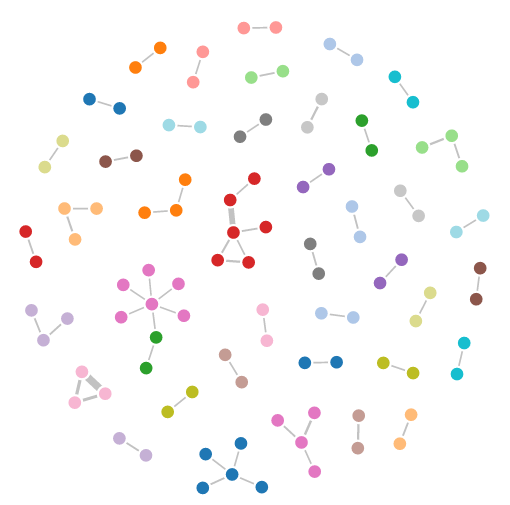
\includegraphics[width=\columnwidth, height=5cm,keepaspectratio]{figure/graph_deteksi}
\caption{Graph Result Community Detection}
\label{graph_community_detection}
\end{figure}

\subsection{Identify Community}
First, we apply equation \ref{eq:tf-idf} to our graph data, where in our case product bought frequency as word frequency \((tf)\) and number of community or customer bought product as number of document containing term \((idf)\), after that we calculate TC score follow equation \ref{eq:TC_score} for each product bought in every community, and then calculate Z-score to removed not an importand product.

There are 15,413 distinct product bought on all community, to simplify, we use Z-score to remove not an importand product. Based on product with z-score more than 0, there are remain 1,075 distinct product to process in next step. After that we calculate TC score for each community, and get product with highest TC score . Table \ref{tab:result_identify_community} show result 3 community with their characteristic product.

\begin{table}[h]
\renewcommand{\arraystretch}{1.3}
\caption{Characteristic Product Community}
\label{tab:result_identify_community}
\centering
\begin{tabular}{|c|p{6cm}|p{1cm}|}
    \hline
    Community  &  Characteristic Product\\
    \hline
    40 & 'Casablanca Outer', 'Asuka Tunik', 'Maldives Top'\\
    \hline
    32 & 'Pearl Glamour Peafowl', 'Inner Zipper Reguler', 'Slimface Inner', 'Daster Tetron Batik', 'Nuna Turbular'\\
    \hline
    6 & 'Alana Shawl', 'Inner Zipper Reguler', 'Grisy Sweatshirt', 'Sam Shawl', 'Laiqa Magazine Vol 25'\\
    \hline
\end{tabular}
\end{table}



\section{Conclusion}
This research attemps to try identify customer community in graph customer e-commerce. We use Girvan-Newman algotihm for community detecton. Community detection result can identified using concept TF-IDF in text mining and to improve identify, we apply feature reduction with Z-score. The result is with apply TF-IDF in graph customer e-commerce, we can get characteristic product in each community. It can support marketing to arrange promotion product to each community.


% conference papers do not normally have an appendix


\begin{thebibliography}{1}


\bibitem{Tsiptsis}
Tsiptsis, K., and Chorianopoulos, A., "Data Mining Techniques in CRM" , Wiley 2009

\bibitem{Malliaros}
Malliaros, F. D., and Vazirgiannis, M., "Clustering and community detection in directed networks: A survey". Physics Reports 2013.

\bibitem{Ahmed}
Ahmed, R. E., Shehab, M., Morsy, S., and Mekawie, N., "Performance study of classification algorithms for consumer online shopping attitudes and behavior using data mining". 2015 Fifth International Conference on Communication Systems and Network Technologies

\bibitem{Newman}
M. E. Newman and M. Girvan, "Finding and evaluating
community structure in networks," Physical Review E,
vol. 69, no. 2, p. 026113, 2004.

\bibitem{Kameyama}
Kameyama, S., Uchida, M., Shirayama, S., "A New Method for Identifying Detected Communities Based on Graph Substructure" 2007 IEEE/WIC/ACM International Conferences on Web Intelligence and Intelligent Agent Technology

\bibitem{Uchida}
M. Uchida, N. Shibata and S. Shirayama,"Identification and Visualization of Emerging Trends from Blogosphere", Proceedings of ISWSM, pp. 305-306 (2007)

\bibitem{Mairisha}
Mairisha, M., "Integration of Coupling Degree Concept for Calculating Modularity in Quality Analysis of
Community Structure Based on Weighted Graph" Master’s Program Thesis, Institut Teknologi Bandung, 2016

\bibitem{Munggaran}
Munggaran. M. Rizky., "Identification of Trending Events From News Using Modified K-means Clustering Technique and Term Contribution Technique", Master’s Program Thesis, Institut Teknologi Bandung, 2016

\bibitem{Dai}
Dai, Xiangying, och Yunlian Sun. "Event Identification within News Topics ." IEEE ,
2010: 978-1-4244-6837-9/10.

\bibitem{DaiX}
Dai, Xiang-Ying, Qing-Cai Chen, Xiao-Long Wang, och Jun Xu. "Online Topic
Detection And Tracking Of Financial News Based On Hierarchical Clustering ."
Proceeding of International Conference on Machine Learning and Cybernetics,
2010: pp. 3341-3346.

\bibitem{Gopalakrishnan}
Gopalakrishnan, K., Balakrishnan, B., and Jordan, R., "Clusters and Communities in Air Traffic Delay Networks", 2016 American Control Conference (ACC)

\bibitem{Liu}
Liu, Tao, Shengping Liu, Zheng Chen, och Wei-Ying Ma. "An Evaluation on Feature
Selection for Text Clustering." Proceedings of the Twentieth International
Conference on Machine Learning, 2003.

\bibitem{Community}
Jahanbakhsh, K. (2016, April). A Python implementation of Girvan-Newman community detection algorithm for weighted graphs. Retrieved July 10, 2016, from https://github.com/kjahan/community/

\bibitem{Olga}
Olga Vechtomova, Stephen Robertson, and Susan Jones, "Query expansion with long-span collocates," Information Retrieval, vol. 6, no. 2, pp. 251-273 , 2003.

\bibitem{Lan}
Lan, Man, och Chew Lim Tan. "Supervised and Traditional Term Weighting Methods for
Automatic Text Categorization ." IEEE PAMI, 2007: VOL. 10, NO. 10.

\end{thebibliography}





% that's all folks
\end{document}


